%----------------------------------------------------------------
%% Template para preparação de trabalho de conclusão de 
%% curso   (TCC)   do   Departamento   de   Economia   da 
%% Universidade      Estadual     de      Londrina       (UEL)
%
%% Autores: 
%% Prof Ph.D. Joanna G. Alexopoulos
%% Prof. Dr. Marcelo S. Bego 
%
%% Data da última atualização: 22/02/2020
%----------------------------------------------------------------
%%
%% Customizações do abnTeX2 (http://abnTeX2.googlecode.com) 
%%
%% Este trabalho pode ser distribuído e/ou modificado sob as
%% condições da Licença Pública do LaTeX Project, versão 1.3.
%% A versão desta licença pode ser encontrada em:
%%   http://www.latex-project.org/lppl.txt
%% e faz parte da versão LaTeX 01/12/2005.
%%
%% Este trabalho tem como status de manutenção LPPL como "maintained".
%% 
%% Os atuais responsáveis por esse trabalho são: 
%% Prof Ph.D. Joanna G. Alexopoulos
%% Prof. Dr. Marcelo S. Bego 
%%
%% Mais informações sobre abnTeX2 estão disponíveis em: 
%%  https://github.com/abntex/abntex2
%%
%----------------------------------------------------------------
%% Sobre a classe abntex2.cls:
%% abntex2.cls, v-1.9.5 laurocesar
%% Copyright 2012-2015 by abnTeX2 group at https://www.abntex.net.br/ 
%%
%----------------------------------------------------------------

\documentclass[12pt,oneside,a4paper,chapter=TITLE,english,brazil,sumario=abnt-6027-2012]{abntex2}

% Dark mode
% \usepackage{xcolor}
% \pagecolor[rgb]{0.1,0.1,0.15} %black
% \color[rgb]{0.5,0.5,0.5} %grey

% %%%%%%%%%%%%%%%%
% PACOTES
% %%%%%%%%%%%%%%%%

\usepackage{lmodern}			
\usepackage[T1]{fontenc}		
\usepackage[utf8]{inputenc}		
\usepackage{indentfirst}		
\usepackage[dvipsnames]{xcolor}				
\usepackage{graphicx}			
\usepackage{microtype} 
\usepackage{multicol}
\usepackage{multirow}
\usepackage{float}	
\usepackage{lipsum}				
\usepackage{tikz}
\usepackage{ragged2e} 
\usepackage[brazilian,hyperpageref]{backref}	
\usepackage[alf]{abntex2cite}
\usepackage{blindtext} 
\usepackage{mathptmx}
\usepackage[labelfont=bf]{caption}
\captionsetup{labelfont=bf}
\usepackage[singlelinecheck=false]{caption}
\usepackage{amsmath}

% %%%%%%%%%%%%%%%%
%MARGENS
%As margens são configuradas conforme a NBR 14724:2011
%As margens devem ser: para o anverso, esquerda e superior de 3 cm e direita e inferior de 2 cm; para o verso, direita e superior de 3 cm e esquerda e inferior de 2 cm. 

% %%%%%%%%%%%%%%%%
%FONTES 
% %%%%%%%%%%%%%%%%

% %%%%%%%%%%%%%%%%
%TIPO DE FONTE
\renewcommand{\sfdefault}{\rmdefault} % Fonte: Times New Roman

% %%%%%%%%%%%%%%%%
% TAMANHO E ESTILO DAS FONTES DOS TÍTULOS E SUBSEÇÕES 
\renewcommand{\ABNTEXchapterfontsize}{\large \bfseries}%14pt

\renewcommand{\ABNTEXsectionfont}{\bfseries}%Subseções em negrito.

% %%%%%%%%%%%%%%%%
% ESPAÇAMENTOS
% %%%%%%%%%%%%%%%%

% TAMANHO DO PARÁGRAFO 
\setlength{\parindent}{3cm} %Primeira linha

%ESPAÇO ENTRE LINHAS
%O padrão é definido como \OnehalfSpacing (1.5)


% %%%%%%%%%%%%%%%%
%INFORMAÇÕES DA CAPA, FOLHA DE ROSTO E FOLHA DE APROVAÇÃO 
% %%%%%%%%%%%%%%%%

% %%%%%%%%%%%%%%%%
%NOME DO TRABALHO 
\titulo{\bfseries ANÁLISE DA DINÂMICA INFLACIONÁRIA SOB O REGIME DE METAS DE INFLAÇÃO NO BRASIL ENTRE 2003 e 2023}


% %%%%%%%%%%%%%%%%
%NOME DO AUTOR 
\autor{LUCAS BONI DOS ANJOS AMARAL ALVARENGA}


% %%%%%%%%%%%%%%%%
%NOME DO ORIENTADOR
\orientador{Carlos Eduardo Caldarelli}


% %%%%%%%%%%%%%%%%
\local{LONDRINA, PARANÁ}
\data{\the\year}
\tipotrabalho{monografia}
\instituicao{Universidade Estadual de Londrina (UEL)}
\preambulo{ Trabalho de Conclusão de Curso apresentado ao Departamento de Economia da Universidade  Estadual de Londrina.}
% %%%%%%%%%%%%%%%%


% %%%%%%%%%%%%%%%%
% CAPA UEL
\renewcommand{\imprimircapa}{
	\begin{capa}
		\center
		\begin{figure}
		
\includegraphics[height=4.5cm,width=14cm]{Logo_UEL}
		\end{figure}

		
\begin{tikzpicture}
		\fill[ForestGreen!90] (17.1,0.6) rectangle (1,1);
		\end{tikzpicture}
		\large 
		
		{\bfseries CENTRO DE ESTUDOS SOCIAIS APLICADOS\\
		DEPARTAMENTO DE ECONOMIA\\
		CURSO DE CIÊNCIAS ECONÔMICAS\\}
		
		
		\vspace{5cm}
		
		{\ABNTEXchapterfont\textsc{\Large\imprimirtitulo}}
		
		\vfill
		
		\begin{flushright}
			{\ABNTEXchapterfont\textsc{\Large \imprimirautor}}
			
		\end{flushright}
		
		
\begin{tikzpicture}
		\fill[ForestGreen!90] (17.1,0.6) rectangle (1,1);
		\end{tikzpicture}
		
		{\imprimirlocal}
		
		{\imprimirdata}
		
	\end{capa}
}

% %%%%%%%%%%%%%%%%
% FOLHA DE ROSTO
\makeatletter

\renewcommand{\folhaderostocontent}{
	\begin{center}
      \large 	
	
	  {\ABNTEXchapterfont\textsc{\Large \imprimirautor}}
		
		\vspace{6cm}
		
		{\ABNTEXchapterfont\textsc{\Large \imprimirtitulo}}
		
		\vspace{2cm}
		
		\begin{flushright}
			\begin{minipage}{8cm}
				\SingleSpacing
				Trabalho de Conclusão de Curso apresentado ao Departamento de Economia da Universidade Estadual de Londrina.
				
				Orientador: Prof. \imprimirorientador
			\end{minipage}%
		\end{flushright}
		
		\vfill
		
		
		{\large\imprimirlocal}
		
		{\large\imprimirdata}
	\end{center}
}
\makeatother


% %%%%%%%%%%%%%%%%
% FOLHA DE APROVAÇÃO 
\makeatother

\newcommand{\folhaDeaprovacao}{
	\begin{center}
		
		\begin{folhadeaprovacao} 
			\begin{center} 
				
					
				
			{\ABNTEXchapterfont\textsc{\large \imprimirautor}}
				
				\vspace{2cm}
				
			{\ABNTEXchapterfont\textsc{\large \imprimirtitulo}}
				
				\vspace{1cm}		
				\begin{flushright}
					\begin{minipage}{10cm}
						\SingleSpacing
						Trabalho de Conclusão de Curso apresentado ao Departamento de Economia da Universidade Estadual de Londrina.
					\end{minipage}%
				\end{flushright}	
				
				\vspace{2cm}
				
				\begin{flushright}
					\begin{minipage}{10cm}		
						\centering
					{\bfseries COMISSÃO EXAMINADORA}
					\end{minipage}
				\end{flushright}	
				
				\vspace{1cm}
				
				\begin{flushright}
					\begin{minipage}{10cm}	
						\centering
						\hrule \hspace{0.2cm}
						
						Orientador(a): Prof(a). \imprimirorientador  
						
						\imprimirinstituicao
					\end{minipage}%
				\end{flushright}
				
				\vspace{1cm}
				
				\begin{flushright}
					\begin{minipage}{10cm}	
						\centering
						\hrule \hspace{0.2cm}
						
						Prof(a). NOME BANCA 1
						
						\imprimirinstituicao
					\end{minipage}%
				\end{flushright}		
				
				
				\vspace{1cm}
				
				\begin{flushright}
					\begin{minipage}{10cm}	
						\centering
						\hrule \hspace{0.2cm}
						
						Prof(a). NOME BANCA 2 
						
						\imprimirinstituicao
					\end{minipage}%
				\end{flushright}
				
				\vfill 
				
				\begin{flushright}
					\begin{minipage}{6cm}	
				\centering
				Londrina, XX de XX de \imprimirdata.
					\end{minipage}
			\end{flushright}
		
			\end{center} 
		\end{folhadeaprovacao}
	\end{center}
}
\makeatother


% %%%%%%%%%%%%%%%%
%REGULAMENTO DO TRABALHO DE CONCLUSÃO DO CURSO DE ECONOMIA (DISCIPLINAS MONOGRAFIA I E II – 6TCC404 E 6TCC405)
% %%%%%%%%%%%%%%%%

%ART.16 A estrutura da monografia compõe-se de:

%I. Capa;
%II. Folha de rosto;
%III. Elementos pré-textuais;
%IV. Resumo e “Abstract” (ou versão em Espanhol ou ainda em Francês):
%V. Sumário;
%VI. Introdução;
%VII. Desenvolvimento, contendo Referencial Teórico ou Econométrico ou Revisão de Literatura ou Revisão Bibliográfica ou Modelo Teórico; e nos casos de estudos quantitativos Metodologia e Fonte e tratamento de dados;
%VIII. Resultados e discussão;
%IX. Considerações finais ou Conclusão;
%X. Referências;
%XI. Anexos e Apêndices, quando for o caso
%%%%%%%%%%%%%%%%%%%%%%%%%%%%



% INÍCIO DO DOCUMENTO
\begin{document}

% Retira espaço extra obsoleto entre as frases.
\frenchspacing 


% %%%%%%%%%%%%%%%%
% CAPA
\imprimircapa

% %%%%%%%%%%%%%%%%
%FOLHA DE ROSTO
\folhaderostocontent


% %%%%%%%%%%%%%%%%
%FIXA CATALOGRÁFICA 
%Incluir fica catalográfica
%\pagebreak


% %%%%%%%%%%%%%%%%
%FOLHA DE APROVAÇÃO 
\folhaDeaprovacao


% %%%%%%%%%%%%%%%%
%DEDICATÓRIA
\begin{dedicatoria}
	\vspace*{\fill}
	\noindent
	Dedico esse trabalho aos meus pais, Bruno e Silvia, por todo amor, apoio e incentivo, que foram fundamentais para a realização de mais uma conquista. Sua dedicação e sacrifícios me proporcionaram a oportunidade de seguir em frente e realizar meus objetivos. 
	\vspace*{\fill}
\end{dedicatoria}


% %%%%%%%%%%%%%%%%
%AGRADECIMENTOS
\begin{agradecimentos}
	\noindent
	Agradeço aos professores e colegas de curso, que contribuíram com conhecimentos, experiências e incentivos, tornando a jornada acadêmica mais rica e gratificante. Aos amigos, que estiveram presentes nos momentos de lazer e de estudo, proporcionando equilíbrio e motivação durante o percurso.	À Universidade Estadual de Londrina por oferecer um ambiente de aprendizado e crescimento. A todos aqueles que, direta ou indiretamente, colaboraram para a conclusão deste trabalho.
\end{agradecimentos}


% %%%%%%%%%%%%%%%%
%RESUMO
\noindent
ALVARENGA, Lucas. {\bfseries Análise da Dinâmica Inflacionária Sob o Regime de Metas de Inflação no Brasil Entre 2003 e 2023}, \imprimirdata. <FOLHAS> f. Monografia (Curso de Ciências Econômicas). Centro de Estudos Sociais Aplicados, Universidade Estadual de Londrina, Londrina, 2024.

\setlength{\absparsep}{18pt} % ajusta o espaçamento dos parágrafos do resumo
\begin{resumo}

	Este trabalho tem por objetivo verificar o impacto da inflação de oferta e da inflação de demanda sobre a economia brasileira e avaliar os efeitos exercidos por estas sobre a eficácia do regime de metas de inflação (RMI) no Brasil. Será examinado se as respostas do Banco Central são eficientes e sob quais óticas a política monetária deve ser definida a fim de atender os objetivos propostos pelo RMI. Por meio deste trabalho, busca-se atingir um melhor entendimento dos mecanismos que regem a dinâmica inflacionária no Brasil e como é moldada a resposta à inflação pela autoridade monetária brasileira.
	
	\textbf{Palavras-chave}: inflação; oferta; demanda
\end{resumo}


% %%%%%%%%%%%%%%%%
%ABSTRACT
\noindent
ALVARENGA, Lucas. {\bfseries Análise da Dinâmica Inflacionária Sob o Regime de Metas de Inflação no Brasil Entre 2003 e 2023}, \imprimirdata. <FOLHAS> f. Monografia (Curso de Ciências Econômicas). Centro de Estudos Sociais Aplicados, Universidade Estadual de Londrina, Londrina, 2024.

\begin{resumo}[Abstract]
	\begin{otherlanguage*}{english}
		
		Write your abstract here... 
		
		\vspace{\onelineskip}
		
		\noindent 
		\textbf{Keywords}: 
	\end{otherlanguage*}
\end{resumo}
\pagebreak


% %%%%%%%%%%%%%%%%
%LISTA DE FIGURAS
\pdfbookmark[0]{\listfigurename}{lof}
\listoffigures*
\cleardoublepage


% %%%%%%%%%%%%%%%%
%LISTA DE TABELAS
\pdfbookmark[0]{\listtablename}{lot}
\listoftables*
\cleardoublepage


% %%%%%%%%%%%%%%%%
%LISTA DE ABREVIATURAS
\begin{siglas}
	\item[UEL] Universidade Estadual de Londrina. 
	\item[ABNT] Associação Brasileira de Normas Técnicas.
	\item[RMI] Regime de metas de inflação
	\item[SELIC] Sistema Especial de Liquidação e Custódia
	\item[IPCA] Índice Nacional de Preços ao Consumidor Amplo
	\item[IGP-DI] Índice Geral de Preços - Disponibilidade Interna
	\item[CMN] Conselho Monetário Nacional
	\item[ECM] Modelagem de Correção de Erros
	\item[VAR] Análise de Vetores Autoregressivos
	\item[PIB] Produto Interno Bruto
	\item[PAI] Programa de Ação Imediata
	\item[PEC] Proposta de Emenda à Constituição
\end{siglas}
\pagebreak


% %%%%%%%%%%%%%%%%
%LISTA DE SíMBOLOS
% \begin{simbolos}
% 	\item[Depeco] Departamento de Economia
% \end{simbolos}
% \pagebreak


% %%%%%%%%%%%%%%%%
% SUMÁRIO
\pdfbookmark[0]{\contentsname}{toc}
\tableofcontents*
\cleardoublepage


% %%%%%%%%%%%%%%%%
%INÍCIO DO TEXTO
\textual % indica o início do texto para a numeração das páginas
\pagestyle{simple}
\aliaspagestyle{chapter}{simple}

\chapter{Introdução}

O controle da inflação é um dos principais desafios enfrentados pelas autoridades econômicas em diversas nações ao redor do mundo. No Brasil, a adoção do Regime de Metas de Inflação (RMI) em 1999 representou uma mudança significativa na condução da política monetária, com o objetivo de estabilizar os preços e promover um ambiente econômico previsível \cite{fraga_2003_inflation}. Diante desse contexto, este trabalho tem como objetivo analisar a dinâmica inflacionária no Brasil sob o RMI entre os anos de 2003 e 2023, focando especificamente nos componentes de inflação de demanda e de oferta para verificar a efetividade das políticas do Banco Central.

Ao longo deste trabalho, serão abordados os diferentes tipos de inflação, seguido por um detalhamento do histórico econômico brasileiro e uma discussão sobre o RMI e a política monetária na terceira seção. A quarta seção detalhará a metodologia, o modelo utilizado e os dados coletados. Os resultados e a discussão serão apresentados na quinta seção, culminando com a conclusão na sexta seção. Por meio desta análise, espera-se contribuir para uma melhor compreensão da dinâmica inflacionária no Brasil e a eficácia do RMI na promoção da estabilidade econômica, assim como os impactos sobre o produto e o desenvolvimento econômico.

Para compreender o cenário a ser estudado, definimos o Regime de Metas de Inflação como um arranjo institucional em que o Banco Central se compromete a manter a inflação dentro de um intervalo preestabelecido, utilizando instrumentos de política monetária, como as operações em \textit{open market}, para alcançar esse objetivo \cite{svensson_1997_inflation}. Este regime busca ancorar as expectativas inflacionárias dos agentes econômicos, contribuindo para a estabilidade macroeconômica \cite{mishkin_2000_inflation}. Desde sua implementação, o RMI no Brasil tem se baseado em metas anuais de inflação definidas pelo Conselho Monetário Nacional (CMN), com o Banco Central ajustando a taxa do Sistema Especial de Liquidação e Custódia (SELIC) via instrumentos de política monetária para controlar a demanda agregada e manter a inflação dentro dos limites estipulados.

De acordo com o Banco Central do Brasil (2013), A taxa SELIC é obtida através do cálculo da taxa média ponderada e ajustada das operações de financiamento de um dia, que são garantidas por títulos públicos federais. Essas operações ocorrem no sistema financeiro ou em câmaras de compensação e liquidação de ativos, sob a forma de operações compromissadas, onde o vendedor se compromete a recomprar os títulos vendidos no dia útil seguinte. Abaixo, na equação 1.1, é dada a fórmula utilizada para o cálculo da taxa.

\begin{equation}
	\left[ \left( \left(\frac{\sum_{j=1}^{n} L_j \cdot V_j}{\sum_{j=1}^{n} V_j} \right)^{252} - 1 \right) \times 100 \right] \textrm{\% ao ano}
\end{equation}


A equação 1.1 baseia-se em três principais variáveis, sendo elas $L_j$, o fator diário correspondente à taxa da j-ésima operação, $V_j$, o valor financeiro correspondente à taxa da j-ésima operação e $n$, o número de operações que compõem a amostra.

É essencial, também, detalhar os diferentes tipos de inflação experienciados pelo país para analisar como o Banco Central tem respondido. A economia brasileira, como muitas outras, está sujeita a um descompasso entre o crescimento real e a base monetária, resultando em inflação. O processo inflacionário pode ter como fonte diversos fatores, sendo comum verificar a inflação de oferta, a inflação de demanda, a inflação inercial e a inflação estrutural. Cada um desses tipos de inflação apresenta características distintas que influenciam a eficácia do RMI.

Como exemplo, a inflação de demanda ocorre quando a demanda por bens e serviços supera a capacidade produtiva da economia, levando a aumentos generalizados de preços \cite{olivierblanchard_2013_macroeconomics}. Por outro lado, a inflação de oferta é impulsionada por choques nos custos de produção, como aumentos nos preços de matérias-primas ou salários \cite{blinder_2008_the}. Compreender a interação entre os tipos de inflação e o funcionamento do RMI é crucial para avaliar a eficácia das políticas monetárias adotadas pelo Banco Central do Brasil nas últimas décadas. Nesse contexto, o presente trabalho pretende investigar como a inflação de demanda e de oferta influenciaram a dinâmica inflacionária no Brasil durante o período analisado e como o RMI respondeu a esses desafios.

Para isso, é essencial utilizar técnicas econométricas aplicadas a séries temporais relacionadas aos índices de preços, produte interno e outros indicadores econômicos. A análise de séries temporais permite modelar e prever o comportamento de variáveis econômicas ao longo do tempo, capturando tanto as tendências quanto as flutuações cíclicas e sazonais \cite{enders_2015_applied}. Métodos como a Análise de Vetores Autoregressivos (VAR), a Modelagem de Correção de Erros (ECM) e os testes de raiz unitária são frequentemente utilizados para investigar a relação entre a política monetária e a inflação \cite{hamilton_2020_time}.

A aplicação de econometria a séries temporais envolve várias etapas, incluindo a identificação e a modelagem das propriedades estocásticas das séries de dados, a estimação dos parâmetros do modelo e a realização de testes de hipóteses para validar os resultados \cite{stock_2020_introduction}. Essas técnicas permitem aos pesquisadores avaliar a resposta da inflação a choques de demanda e oferta, bem como a eficácia das intervenções do Banco Central no controle dos preços. A seguir, é feita a descrição aprofundada dos tipos de inflação que a economia brasileira observou historicamente e sua relação com o RMI.

\chapter{Tipos de Inflação}

% TODO: Bresser-Pereira (1990) afirma que no caso brasileiro o gatilho da hiperinflação foi a crise fiscal nos anos 80 que pode ser dividida em três componentes: o déficit público, a dívida pública, tanto interna quanto externa e o curto prazo de vencimento dos títulos públicos.

Historicamente, o Brasil enfrentou diferentes tipos de inflação, cada uma influenciada por fatores econômicos e contextos específicos. Nos anos 1980 e início dos anos 1990, o país sofreu com altos níveis de inflação, caracterizada por aumentos de preços extremamente rápidos e incontroláveis. Esse período foi marcado por políticas econômicas instáveis, déficits fiscais elevados e um ciclo de indexação de preços, onde os preços e salários eram ajustados automaticamente à inflação passada, perpetuando o ciclo inflacionário. Diversos planos econômicos foram implementados, como o Plano Cruzado, Plano Bresser e os dois planos Collor, mas falharam em conter a inflação de forma sustentável.

O Brasil experenciou de forma ostensiva a inflação inercial no final do sécula XX. Esse fenômeno é como um ciclo vicioso, uma vez que a inflação persiste devido à expectativa de que ela continuará, independentemente de outros fatores econômicos. Nos anos 1990, especialmente antes do Plano Real, a inflação inercial era alimentada pela indexação, onde preços e contratos eram ajustados automaticamente com base na inflação passada. O Plano Real, implementado em 1994, conseguiu quebrar essa inércia ao introduzir uma nova moeda e uma série de reformas econômicas que estabilizaram a economia. A partir desse ponto, o Brasil passou a experimentar uma inflação mais controlada, embora ainda enfrentasse desafios ocasionais devido a choques externos e flutuações internas na economia.

% TODO: Criar tabela com 

\section{Inflação de Oferta}

% TODO: Citar como o RMI corrije esse tipo de situação e porque isso pode ser problemático

% TODO: A inflação de custos, além de elevar o nível de preços da economia, causa estagflação, expressão empregada quando a economia apresenta alto nível de preços e contração do produto interno bruto, diferentemente da inflação de demanda, onde a expansão da demanda agregada, além de elevar o nível de preços, aquece a economia e estimula o crescimento do PIB.

Um exemplo marcante de inflação de oferta, tanto no Brasil quanto no mundo, ocorreu durante as crises do petróleo dos anos 1970. O aumento abrupto dos preços do petróleo, um insumo fundamental para diversas indústrias, resultou em custos mais altos de transporte e produção, impactando a economia brasileira. Outro exemplo mais recente foi observado durante a crise hídrica na região sudeste em 2014 e 2015, quando a escassez de água afetou a produção agrícola e a geração de energia hidrelétrica, levando ao aumento dos custos de alimentos e eletricidade (FRANCO, 2014).

Também conhecida como inflação de custos, esse tipo de inflação ocorre quando os custos de produção aumentam, levando a um aumento nos preços dos bens e serviços finais. Esses aumentos nos custos podem ser decorrentes de elevações nos preços das matérias-primas, aumentos salariais, ou choques de oferta adversos, como desastres naturais ou interrupções no fornecimento de insumos essenciais. \citeonline{blinder_2008_the} descrevem a inflação de custos como um fenômeno onde os produtores, enfrentando maiores custos de produção, repassam esses custos para os consumidores através de preços mais altos.

Combater a inflação de oferta envolve várias estratégias, incluindo a melhoria da infraestrutura para reduzir custos de produção e distribuição, a diversificação de fontes de insumos para diminuir a dependência de um único fornecedor e o incentivo à inovação e adoção de novas tecnologias para aumentar a produtividade. Além disso, políticas cambiais que estabilizem a moeda podem minimizar os impactos de variações cambiais nos custos de insumos importados. 

\section{Inflação de Demanda}

Se por um lado choques nos custos de produção e salários causam inflação de oferta, a inflação de demanda ocorre quando a demanda agregada por bens e serviços supera a capacidade produtiva da economia, resultando em pressões inflacionárias. Este tipo de inflação é frequentemente associado a períodos de crescimento econômico robusto, onde a renda disponível e o consumo das famílias aumentam significativamente. Segundo \citeonline{olivierblanchard_2013_macroeconomics}, a inflação de demanda pode ser desencadeada por políticas fiscais expansionistas, como aumentos nos gastos governamentais ou cortes de impostos, que elevam a demanda agregada sem um correspondente aumento na oferta.

Um exemplo histórico significativo de inflação de demanda ocorreu durante a década de 1970, quando muitos países enfrentaram pressões inflacionárias devido a políticas fiscais expansionistas e aumentos rápidos nos gastos de consumo \cite{blinder_2008_the}. No Brasil, a inflação de demanda tem sido uma preocupação constante, especialmente em contextos de políticas fiscais agressivas que aumentam o poder de compra sem um acompanhamento na produção. Segundo \cite{woodford_2009_interest}, a gestão eficaz da demanda agregada é crucial para evitar pressões inflacionárias, destacando a importância da coordenação entre políticas fiscais e monetárias. Portanto, o controle da inflação de demanda requer uma abordagem equilibrada que inclua a moderação das expansões fiscais e uma política monetária prudente que consiga antecipar e neutralizar excessos de demanda.

% TODO: Falar mais sobre o RMI e seus impactos

Uma das principais ferramentas utilizadas na gestão macroeconômica brasileira é o aumento das taxas de juros, que desestimula o consumo e o investimento ao encarecer o crédito. Além disso, a redução dos gastos públicos e o aumento da tributação podem diminuir a quantidade de dinheiro em circulação, ajudando a conter a demanda agregada. Essas medidas visam equilibrar a demanda com a capacidade produtiva da economia, reduzindo a pressão sobre os preços.

\section{Inflação Estrutural}

Diferentemente das modalidades anteriores, a inflação estrutural é causada por desequilíbrios fundamentais na estrutura econômica de um país. Fatores como a rigidez dos mercados, a ineficiência produtiva e a falta de competitividade em determinados setores podem contribuir para esse tipo de inflação. A inflação estrutural é particularmente relevante em economias em desenvolvimento, onde a infraestrutura inadequada e a baixa produtividade agrícola podem levar a aumentos persistentes nos preços. Essa forma de inflação requer reformas estruturais profundas para melhorar a eficiência e a capacidade produtiva da economia.

No Brasil, a inflação estrutural pôde ser observada durante as décadas de 1970 e 1980, quando o país enfrentou uma inflação persistente devido a vários fatores estruturais na economia. Entre esses fatores estavam a ineficiência produtiva, a baixa competitividade das indústrias nacionais, a excessiva burocracia, e a rigidez do mercado de trabalho. Isso foi agravado pela indexação generalizada da economia, onde salários, contratos e preços eram ajustados automaticamente com base na inflação passada, criando um ciclo contínuo de reajustes que perpetuava a inflação.

\section{Inflação Inercial}

% TODO: Como retratam Giambiagi et al. (2011), no Plano Collor II houve a tentativa de controle da inflação por meio do congelamento dos preços, visando acabar com a memória inflacionária, ou seja, desindexar a economia, contudo o plano reduziu a inflação somente no curto prazo, a solução veio com o Plano Real em 1994 que estabeleceu a Unidade Real de Valor (URV) para desindexar a economia e determinou o lançamento de uma nova unidade monetária que estaria indexada ao dólar, nascia assim o real.

Outra forma de inflação experenciada pelo Brasil na mesma época foi a inflação inercial, que é associada à tendência dos índices de preços continuarem subindo devido à persistência das expectativas inflacionárias passadas. Esse tipo de inflação é mantido pela indexação de preços e salários, onde os agentes econômicos ajustam automaticamente os preços e salários futuros com base na inflação passada. \citeonline{lopes_1985_inflao} explica que, em um ambiente de inflação inercial, as expectativas de inflação se tornam autorrealizáveis, perpetuando a continuidade da inflação mesmo na ausência de novos choques de demanda ou custos.

A indexação da economia, como já mencionada na seção 2.3 de inflação estrutural, fazia com que o ajuste automático dos salários e contratos com base na inflação passada criasse um ciclo contínuo de reajustes. Essa indexação fazia com que a inflação se perpetuasse ao longo do tempo, principalmente nos anos de 1980, quando esse comportamento começou a ser identificado a partir do desenvolvimento de teorias a respeito (PEREIRA, 1998).

% TODO: Os efeitos sobre a distribuição de renda são um dos mais graves efeitos da inflação, conforme Gremaud, Vasconcellos e Toneto Júnior (2007) e Blanchard (2011) alientam, a desigualdade é acentuada quando a taxa de crescimento dos preços não acomete todos os componentes da economia no mesmo ritmo, quando os preços de bens e serviços sobem a um determinado ritmo e o salário não acompanha faz com que a parcela mais pobre da população tenha seus orçamentos ainda mais reduzidos.

\chapter{Elementos Sobre Economia Brasileira}

Nessa seção, inicia-se a contextualização da história econômica do Brasil, assim como a análise do comportamento da política monetária ao longo do tempo. É feito, também, um detalhamento das principais características das políticas econômicas conduzidas por cada governo de 2003 a 2023 e seus impactos sobre o cenário econômico nacional.

\section{Governos do Século XX}

% TODO: O cenário econômico brasileiro entre a década de 80 e 90 foi marcado por anos de inflação recorrente, o regime militar deixara uma dívida externa estratosférica para os governos seguintes que tinham como principal meta o controle dos preços por meio de planos de estabilização. Sabe-se que todos os planos fracassaram na tentativa de conter o avanço da inflação, como explicam Moran e Witte (1993, p. 120): “No Brasil, são notórias as tentativas de conter este processo, a maioria não obteve o sucesso desejado por vários motivos. [...] dentre os quais destacam o Plano Cruzado I, o Plano Cruzado II, o Plano Bresser, o Plano Verão, o Plano Collor I e o Plano Collor II.”.

A bagagem econômica herdada dos diversos governos do século XX no Brasil teve um impacto duradouro na economia e na capacidade do país de implementar políticas macroeconômicas eficazes. Durante as décadas de 1950 e 1960, os governos de Getúlio Vargas e Juscelino Kubitschek adotaram políticas desenvolvimentistas que promoveram a industrialização acelerada e a expansão da infraestrutura, muitas vezes financiadas por meio de déficit público \cite{bielschowsky_2022_a}. Essas políticas resultaram em um crescimento econômico robusto, mas também em um aumento significativo da dívida pública e das pressões inflacionárias.

Sob o governo de Getúlio Vargas, a criação da Petrobras e da Companhia Siderúrgica Nacional (CSN) marcou um período de forte intervenção estatal na economia. O Estado Novo de Vargas (1937-1945) e seu segundo governo (1951-1954) buscaram consolidar a indústria de base no Brasil, visando reduzir a dependência de importações e fortalecer o mercado interno. Embora essas iniciativas tenham contribuído para a modernização da economia brasileira, elas também levaram a um aumento dos gastos públicos e ao crescimento da dívida externa \cite{fabiogiambiagi_2016_economia}.

Durante o governo de Juscelino Kubitschek (1956-1961), a política econômica se concentrou no Plano de Metas, que buscava ``50 anos em 5'' de desenvolvimento. Esse plano incluiu a construção de Brasília, a nova capital federal, e a expansão da infraestrutura de transporte e energia. Embora esses projetos tenham impulsionado a industrialização e o crescimento econômico, eles também resultaram em um aumento significativo do déficit público e da inflação \cite{bielschowsky_2022_a}. A rápida expansão foi financiada por meio de empréstimos externos, deixando o país vulnerável a crises de balanço de pagamentos.

Nos anos de 1960, a instabilidade política e econômica levou ao golpe militar de 1964, que instaurou um regime autoritário com uma nova agenda econômica. O governo militar inicial adotou medidas de austeridade para controlar a inflação e estabilizar a economia. Contudo, o período mais notável de crescimento, conhecido como o "milagre econômico brasileiro" (1968-1973), foi caracterizado por investimentos massivos em infraestrutura e pela abertura econômica. Esse crescimento foi impulsionado por políticas fiscais e monetárias expansivas, que, embora tenham gerado um aumento substancial do produto interno bruto (PIB), também ampliaram a dívida externa e interna \cite{amaurypatrickgremaud_2009_economia}.

O ``milagre econômico'' foi marcado por grandes projetos, como a construção da Rodovia Transamazônica e a usina de Itaipu, que demandaram enormes recursos financeiros. Embora esses projetos tenham impulsionado a economia, eles também aumentaram as pressões inflacionárias. Além disso, a concentração de renda e a repressão aos movimentos sociais geraram tensões sociais significativas. O choque do petróleo de 1973 exacerbou as vulnerabilidades econômicas, pois aumentou os custos de importação de energia e pressionou ainda mais a balança de pagamentos.

Isso fez com que a década de 1980, chamada de ``década perdida'', fosse marcada por estagnação econômica, hiperinflação e crise da dívida externa. A política econômica dos governos militares posteriores, particularmente sob a presidência de João Figueiredo (1979-1985), foi incapaz de lidar com as consequências dos choques externos e das políticas expansionistas anteriores. A moratória da dívida em 1987 simbolizou a profundidade da crise econômica \cite{fabiogiambiagi_2016_economia} na época. As tentativas de estabilização, como o Plano Cruzado (1986) durante o governo de José Sarney, falharam em resolver os problemas estruturais e levaram a surtos de hiperinflação.

O Plano Cruzado tentou controlar a inflação por meio do congelamento de preços e salários e da introdução de uma nova moeda, o cruzado. Inicialmente, o plano teve sucesso em reduzir a inflação, mas a falta de controle sobre os gastos públicos e a resistência política levaram ao seu fracasso. A inflação retornou, exacerbada pela falta de ajustes estruturais e pela deterioração das contas públicas \cite{fabiogiambiagi_1999_a}.

A transição para a democracia em 1985 trouxe novos desafios econômicos. O governo de Fernando Collor (1990-1992) implementou o Plano Collor, que incluía o confisco de depósitos bancários e a tentativa de liberalização econômica. Embora tenha reduzido temporariamente a inflação, o plano causou uma grave recessão econômica e enfrentou forte oposição política, resultando em sua rápida deterioração e na posterior hiperinflação \cite{lacerda_2010_economia}.

Durante o governo de Itamar Franco (1992-1995), o Brasil finalmente começou a estabilizar sua economia com o Plano Real, liderado pelo então Ministro da Fazenda Fernando Henrique Cardoso. O plano introduziu uma nova moeda, o real, e implementou âncoras cambiais e políticas fiscais rígidas. Essas medidas conseguiram estabilizar a inflação e criar uma base para o crescimento econômico sustentável. O sucesso do Plano Real foi um ponto de inflexão na história econômica do Brasil, marcando o fim de um ciclo de políticas populistas e instabilidade econômica \cite{lacerda_2010_economia}.

A instabilidade econômica e a subsequente estabilização pela qual o Brasil passou no período anterior e posterior ao Plano Real é claramente observada nas variações do Índice Geral de Preços - Disponibilidade Interna (IGP-DI). A Figura 1, a seguir, apresenta a série temporal do comportamento da inflação entre 1985 e 1996 no Brasil, com destaque para as diversas tentativas de estabilização realizadas.

\begin{figure}[H]
	
	\caption{Comportamento da Inflação Mensal - IGP-DI - 1985-1996 (\%)}
	
	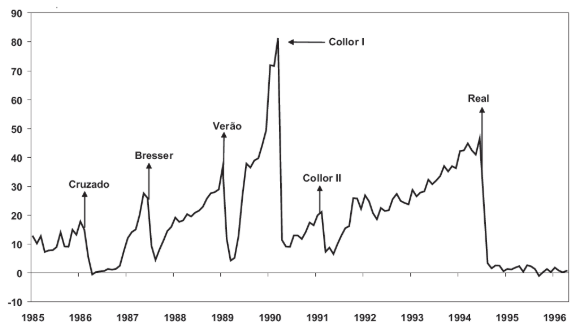
\includegraphics[]{igp-di.png}\\
	
	\footnotesize Fonte: FGV.
	
\end{figure}

Com destaque, a inflação no Brasil (Figura 1), observou diversos choques resultantes de políticas ineficazes no controle dos preços. O legado dos governos populistas do século XX, com suas políticas desenvolvimentistas e intervenções estatais, deixou uma economia caracterizada por altas taxas de inflação, dívida pública crescente e instabilidade macroeconômica. A implementação do RMI em 1999 representou um esforço para romper com esse passado e adotar uma política monetária mais disciplinada e previsível, visando garantir a estabilidade de preços e promover o crescimento sustentável a longo prazo \cite{amaurypatrickgremaud_2009_economia}.

\section{Transição para a Estabilidade: Plano Real e a Introdução do RMI}

O Plano Real, implementado em 1994 durante o governo de Itamar Franco e sob a liderança do então Ministro da Fazenda Fernando Henrique Cardoso, marcou um ponto de inflexão na luta contra a inflação no Brasil. O plano envolveu uma série de medidas macroeconômicas, incluindo a criação de uma nova moeda, o real, a introdução de âncoras cambiais e a implementação de políticas fiscais rigorosas \cite{amaurypatrickgremaud_2009_economia}. Essas medidas conseguiram estabilizar a inflação e restaurar a confiança na economia brasileira.

A estabilidade alcançada pelo Plano Real criou as condições necessárias para a adoção do Regime de Metas de Inflação (RMI) em 1999. Esse novo regime, que enfatiza a transparência e a credibilidade das políticas monetárias, representou uma mudança de paradigma na abordagem do Brasil ao controle da inflação. Ao focar em metas de inflação como guia principal para a política monetária, o Banco Central do Brasil conseguiu ancorar as expectativas inflacionárias e promover um ambiente macroeconômico mais estável.

A implementação do Plano Real começou com uma série de medidas preparatórias, conhecidas como o Programa de Ação Imediata (PAI), que visavam reduzir a inércia inflacionária e estabilizar a economia antes da introdução da nova moeda. Essas medidas incluíram o ajuste fiscal, a redução do déficit público e a liberalização do comércio. Em julho de 1994, o real foi finalmente introduzido, substituindo o cruzeiro real a uma taxa de paridade inicial de 1:1 com o dólar norte-americano. A âncora cambial foi uma ferramenta crucial para estabilizar as expectativas inflacionárias e fortalecer a credibilidade da nova moeda \cite{silva_2002_plano}. 

A introdução do real foi acompanhada por uma política monetária restritiva, com altas taxas de juros para controlar a demanda agregada e evitar pressões inflacionárias. O governo também adotou um regime de câmbio fixo, permitindo que o Banco Central interviesse para manter a paridade da moeda. Essas medidas foram fundamentais para o sucesso inicial do Plano Real, que conseguiu reduzir a inflação anual de mais de 2.000\% em 1993 para menos de 10\% em 1996 \cite{fabiogiambiagi_1999_a}.

O sucesso do Plano Real não foi isento de desafios. A âncora cambial, enquanto eficaz no curto prazo, gerou pressões sobre a balança de pagamentos do Brasil, levando a um aumento do déficit em conta corrente. Além disso, a apreciação do real tornou as exportações brasileiras menos competitivas, aumentando a dependência de capital externo para financiar o déficit. Esses desequilíbrios se tornaram evidentes durante as crises financeiras internacionais da segunda metade da década de 1990, como a crise do México (1994-1995), a crise asiática (1997) e a crise da Rússia (1998) \cite{santna_2002_crises}.

Em resposta a essas crises e às pressões cambiais crescentes, o governo brasileiro decidiu abandonar a âncora cambial em janeiro de 1999 e adotar um regime de câmbio flutuante. Essa mudança foi acompanhada pela introdução do Regime de Metas de Inflação (RMI), que visava ancorar as expectativas inflacionárias por meio da transparência e previsibilidade das ações do Banco Central. Sob o RMI, o Conselho Monetário Nacional estabelece metas de inflação anuais, e o Banco Central utiliza as operações de \textit{open market}, redesconto e depósito compulsório como  principais instrumentos para atingir essas metas.

% TODO: No segundo mandato de FHC, entre 1999 e 2002, o país precisou recorrer ao Fundo Monetário Internacional (FMI) para enfrentar o problema externo, recebendo acote de ajuda em torno de U$ 40 bilhões. O acordo com o FMI enfrentou duas adversidades, Giambiagi et al. (2011) explicam que a desconfiança referente a não desvalorização do câmbio por parte do mercado e o desprezo pelo Congresso com relação a medida de contribuição previdenciária, imposta pelo plano, levou a rejeição da medida pelos congressistas e aumentou o pessimismo, acelerando o processo de perda de divisas.

A transição para o RMI representou uma mudança significativa na política monetária do Brasil. Ao invés de se concentrar exclusivamente no controle do câmbio, o Banco Central passou a focar na estabilidade de preços como seu principal objetivo. Essa abordagem permitiu uma maior flexibilidade na condução da política monetária, facilitando a resposta a choques econômicos internos e externos. A transparência do regime de metas também aumentou a credibilidade das políticas do Banco Central, ajudando a ancorar as expectativas inflacionárias e a reduzir a inflação de forma sustentável.

Nos primeiros anos do RMI, a economia brasileira enfrentou desafios significativos, incluindo uma crise cambial em 1999 e um cenário internacional adverso. No entanto, a política monetária firme e a disciplina fiscal contribuíram para a estabilização da economia. A inflação, que chegou a 8,9\% em 1999, foi gradualmente reduzida, atingindo 5,97\% em 2002. A credibilidade do Banco Central e a eficácia do RMI foram reforçadas pela consistência das políticas adotadas, mesmo diante de adversidades \cite{fabiogiambiagi_1999_a}.

Os governos de Fernando Henrique Cardoso (1995-2002) implementaram reformas estruturais importantes que complementaram a estabilidade macroeconômica promovida pelo Plano Real e pelo RMI. Entre essas reformas estavam a privatização de empresas estatais, a liberalização do mercado financeiro e a promoção de ajustes fiscais. Essas medidas contribuíram para aumentar a eficiência econômica e trazer ao Brasil características mais semelhantes às de países desenvolvidos \cite{fabiogiambiagi_2016_economia}.

No início dos anos 2000, o Brasil começou a colher os frutos das reformas e da estabilidade macroeconômica. A economia cresceu, a inflação permaneceu sob controle e a dívida pública passou a ser mais controlada. Apesar de parte do crescimento ter sido eclipsado pela crise energética de 2001 \cite{fabiogiambiagi_2016_economia}, as reformas monetárias foram um sucesso.

Em resumo, a transição para a estabilidade econômica no Brasil foi marcada pela implementação bem-sucedida do Plano Real e a adoção do Regime de Metas de Inflação. Essas mudanças representaram um rompimento com o passado de instabilidade e políticas populistas, estabelecendo as bases para um crescimento econômico sustentável e uma maior credibilidade das instituições econômicas brasileiras. A disciplina fiscal, a independência do Banco Central e a transparência das políticas monetárias foram elementos-chave para o sucesso dessa transição, que continua a influenciar positivamente a economia brasileira até os dias de hoje.

A partir de 2003, a economia brasileira passou por diversas mudanças econômicas e políticas que influenciaram a condução e os resultados do RMI. Os períodos analisados a seguir foram marcados por diferentes administrações que implementaram políticas econômicas distintas, refletindo na dinâmica inflacionária e na eficácia do regime. A seguir, é detalhada a evolução do quadro econômico brasileiro ao longo das diversas gestões.

\section{Período Lula (2003-2010)}

Durante o governo de Luiz Inácio Lula da Silva (2003-2010), o Brasil experimentou um período de forte crescimento econômico, impulsionado pela alta nos preços das \textit{commodities} e um aumento significativo nos investimentos estrangeiros diretos. A gestão do Banco Central, sob a liderança de Henrique Meirelles, manteve uma política monetária rigorosa para controlar a inflação. A taxa SELIC foi usada de forma ativa para garantir que a inflação permanecesse dentro das metas estabelecidas pelo Conselho Monetário Nacional (CMN). Segundo \citeonline{silva_2016_politica}, a política fiscal contracionista adotada nos primeiros anos do governo Lula contribuiu para a credibilidade dos mandatos, permitindo uma redução gradual da taxa de juros sem comprometer a estabilidade dos preços.

O período também foi marcado por um aumento na credibilidade internacional do Brasil, com a economia apresentando crescimento robusto e uma significativa redução na vulnerabilidade externa. O superávit primário foi mantido, garantindo um controle mais rígido das contas públicas e contribuindo para a estabilidade macroeconômica. A combinação de uma política fiscal responsável com uma política monetária eficiente permitiu que o Brasil navegasse com sucesso por um cenário econômico global inicialmente favorável, mas que se tornou desafiador com a crise financeira de 2008 \cite{fabiogiambiagi_2016_economia}.

A crise financeira global de 2008 representou um grande desafio para a economia brasileira. O governo Lula, em resposta, adotou uma série de medidas para mitigar os impactos da crise, incluindo a redução da taxa SELIC e a implementação de pacotes de estímulo fiscal para sustentar o consumo e o investimento. Essas medidas, associadas à robustez do sistema financeiro brasileiro e à atuação prudente do Banco Central, permitiram que o Brasil enfrentasse a crise de maneira mais resiliente em comparação com muitas outras economias emergentes e desenvolvidas.

Além das políticas de estabilização econômica, o governo Lula implementou programas sociais de grande alcance, como o Bolsa Família, que contribuíram para a redução da pobreza e da desigualdade social. Esses programas tiveram um efeito positivo no aumento da demanda interna, apoiando o crescimento econômico. A inclusão social promovida por esses programas não apenas melhorou as condições de vida de milhões de brasileiros, mas também criou um mercado consumidor interno mais dinâmico, o que foi fundamental para o crescimento sustentado da economia durante esse período.

No entanto, o aumento do consumo e a expansão dos programas sociais também colocaram pressão sobre a inflação. A execução do RMI levantou críticas sobre os altos custos dos empréstimos e o impacto negativo sobre o investimento e o crescimento econômico a longo prazo. Dessa forma, o regime de metas de inflação trouxe impactos para a economia brasileira durante o governo Lula, proporcionando estabilidade de preços, mas também impondo restrições à flexibilidade econômica.

% TODO: passar citações para refs.bib

\section{Período Dilma Rousseff (2011-2016)}
O governo de Dilma Rousseff (2011-2016) enfrentou desafios econômicos significativos, incluindo uma desaceleração econômica e aumento das pressões inflacionárias. A política econômica adotada durante este período foi caracterizada por uma expansão fiscal e intervenções frequentes nos preços administrados, como combustíveis e energia, o que dificultou o controle da inflação. A credibilidade do governo foi colocada em questão devido ao uso de medidas não convencionais e à percepção de interferência política no Banco Central. Como resultado, a inflação frequentemente excedeu as metas estabelecidas, exigindo aumentos abruptos na taxa de juros para tentar trazer a inflação de volta ao intervalo meta \cite{carvalho_2016_growth}.

A implementação de políticas expansionistas, conhecidas como "nova matriz econômica", buscava incentivar o crescimento econômico através do aumento dos gastos públicos e subsídios a setores estratégicos. No entanto, essas políticas resultaram em um aumento do déficit fiscal e da dívida pública, o que elevou as expectativas inflacionárias. As desonerações tributárias e a política de controle de preços contribuíram para a deterioração das contas públicas e limitaram a capacidade do Banco Central de utilizar a política monetária para controlar a inflação de maneira eficaz.

O contexto internacional também influenciou significativamente a economia brasileira durante o governo Dilma. A queda nos preços das \textit{commodities} e a desaceleração do crescimento global impactaram negativamente a balança comercial brasileira, reduzindo as receitas de exportação e aumentando a vulnerabilidade externa do país. Esses fatores externos, aliados às políticas domésticas expansionistas, intensificaram as pressões inflacionárias e tornaram o ambiente econômico mais desafiador para a manutenção da estabilidade dos preços.

A falta de coordenação entre as políticas fiscal e monetária foi um dos principais problemas enfrentados durante esse período. Enquanto o Banco Central tentava controlar a inflação através do aumento da taxa SELIC, a política fiscal expansionista do governo gerava pressões contrárias, dificultando o alcance das metas inflacionárias. Esse descompasso entre as políticas minou a eficácia do RMI e aumentou a incerteza econômica, afetando negativamente a confiança dos investidores e consumidores.

Ao final do segundo mandato de Dilma Rousseff, a economia brasileira enfrentava uma grave recessão, com inflação elevada e desemprego em alta. A crise política e econômica culminou no \textit{impeachment} da presidente em 2016. A gestão subsequente herdou um cenário econômico complexo, marcado pela necessidade urgente de ajustes fiscais e de recuperação da credibilidade. Esse período evidenciou a importância de uma coordenação eficaz entre as políticas fiscal e monetária para a manutenção da estabilidade econômica e do controle inflacionário.

\section{Período Michel Temer (2016-2018)}

Com a chegada de Michel Temer à presidência em 2016, houve uma mudança significativa na política econômica do Brasil. Após o \textit{impeachment} de Dilma Rousseff, o governo Temer buscou implementar uma série de reformas estruturais com o objetivo de restaurar a confiança dos mercados e estabilizar a economia brasileira. Entre as principais medidas adotadas estavam a reforma trabalhista e a  proposta de emenda à constituição (PEC) do teto dos gastos, que limitou o crescimento dos gastos públicos à taxa de inflação do ano anterior por vinte anos. Essas reformas foram vistas como cruciais para o ajuste fiscal e para a recuperação da credibilidade econômica do país.

A gestão do Banco Central sob a liderança de Ilan Goldfajn foi marcada por um compromisso firme com o controle da inflação e a estabilização macroeconômica. Uma das primeiras ações de Goldfajn foi ancorar as expectativas inflacionárias, o que permitiu uma redução gradual e consistente da taxa SELIC ao longo de seu mandato. Essa abordagem contribuiu significativamente para a redução da inflação, que voltou a se situar dentro das metas estabelecidas pelo Conselho Monetário Nacional (CMN) após os elevados índices registrados no final do governo Dilma Rousseff.

Além das reformas estruturais e da política monetária rigorosa, o governo Temer também enfrentou o desafio de recuperar a confiança dos investidores e reverter a recessão econômica. O impacto positivo dessas medidas começou a ser percebido já em 2017, quando o Brasil registrou um leve crescimento econômico após dois anos de recessão profunda. A combinação de um ambiente regulatório mais favorável e de uma política monetária estável ajudou a atrair investimentos e a estimular a recuperação do emprego e da renda.

No entanto, o governo Temer também enfrentou dificuldades, incluindo a resistência política às reformas e os escândalos de corrupção que marcaram seu mandato. Apesar das controvérsias, a continuidade da política econômica voltada para a austeridade fiscal e a estabilidade monetária foi fundamental para consolidar os avanços obtidos na estabilização da economia.

\section{Período Jair Bolsonaro (2019-2022)}

O governo de Jair Bolsonaro (2019-2022) enfrentou desafios econômicos significativos, incluindo a pandemia de COVID-19, que impactou profundamente a economia global e doméstica. A resposta inicial do governo incluiu medidas fiscais expansivas para mitigar os efeitos econômicos da pandemia, como o auxílio emergencial e programas de manutenção de emprego, o que aumentou as preocupações inflacionárias. Essas medidas, apesar de essenciais para a proteção social e a manutenção da renda, pressionaram as contas públicas e elevaram a relação dívida/PIB do país.

Durante esse período, Roberto Campos Neto, presidente do Banco Central, manteve uma postura vigilante, ajustando a taxa SELIC conforme necessário para conter as pressões inflacionárias. Inicialmente, a taxa de juros foi reduzida para níveis historicamente baixos a fim de estimular a economia (2\%), mas a partir de 2021, devido ao aumento das pressões inflacionárias, houve um ciclo de elevação da SELIC para controlar a inflação, gerando uma alta significativa (13,75\%).

A pandemia também causou disrupções significativas nas cadeias de suprimentos globais, resultando em aumentos nos preços dos alimentos, energia e outros bens essenciais. Esses choques de oferta, combinados com uma depreciação cambial significativa, contribuíram para o aumento da inflação no Brasil. Apesar dessas dificuldades, o Banco Central adotou medidas de política monetária para evitar que a inflação se descontrolasse, influenciando proativamente a taxa de juros.

A política fiscal do governo Bolsonaro, particularmente durante a pandemia, foi caracterizada por um aumento substancial nos gastos públicos para enfrentar a crise sanitária e econômica. No entanto, essa expansão fiscal foi acompanhada de uma preocupação crescente com a sustentabilidade das contas públicas. A combinação de um elevado déficit fiscal e a crescente dívida pública gerou incertezas sobre a capacidade do governo de cumprir as metas fiscais e de manter a estabilidade econômica a longo prazo.

Além dos desafios econômicos, o governo Bolsonaro também enfrentou uma série de crises políticas que impactaram a economia. A relação tensa entre o poder executivo e os outros poderes, além das constantes mudanças nos ministérios, contribuiu para um ambiente de incerteza. No entanto, a independência formal do Banco Central, conquistada em 2021, foi vista como um passo importante para fortalecer o RMI e garantir uma política monetária mais eficiente e menos sujeita a pressões políticas, contribuindo para a estabilidade macroeconômica.

\section{Perspectivas Recentes e Desafios (2023)}

À medida que o Brasil entra em 2023, enfrenta uma série de desafios e oportunidades econômicas. Um dos principais focos continua sendo o controle da inflação, que permanece uma preocupação central para o Banco Central. Sob a liderança de Roberto Campos Neto, a política monetária tem sido rigorosamente ajustada para garantir que a inflação fique dentro das metas estabelecidas, apesar das pressões inflacionárias globais e domésticas.

% \section{}

% A alta taxa de juros necessária para manter a inflação sob controle tem um impacto negativo sobre o crescimento econômico e o emprego. Os custos de empréstimos elevados desincentivam investimentos e consumo, limitando o crescimento do PIB

% A pressão para atingir metas anuais pode levar a uma política monetária excessivamente restritiva ou expansiva, prejudicando a estabilidade econômica de longo prazo. A tentativa de atingir metas de curto prazo pode negligenciar problemas estruturais mais profundos na economia brasileira

% Dominancia fiscal?

\chapter{Metodologia}

\section{Modelo}

\section{Dados}

\chapter{Considerações Finais}



%%%%%%%%%%%%%
%BIBLIOGRAFIA
\bibliographystyle{abntex2-alf}
\bibliography{ref}



%%%%%%%%%%%%%%%%%
%APÊNCICES
% \apendices

% \chapter{Anexos e Apêndices, quando for o caso.}

% \chapter{Cronograma}

% \begin{table}[H]
% 	\centering
% 	\caption{Cronograma}
% 	\begin{tabular}{|c|c|c|c|c|c|c|c|c|c|c|c|}
% 		\toprule
% 		Atividades\textbackslash{}Data & Jan & Fev & Mar & Abr & Mai & Jun & Jul & Ago & Set & Out & Nov \\
% 		\midrule
% 		Atividade 1                    &     &     &     &     &     &     &     &     &     &     &     \\
% 		\midrule
% 		Atividade 2                    &     &     &     &     &     &     &     &     &     &     &     \\
% 		\midrule
% 		                               &     &     &     &     &     &     &     &     &     &     &     \\
% 		\midrule
% 		                               &     &     &     &     &     &     &     &     &     &     &     \\
% 		\midrule
% 		                               &     &     &     &     &     &     &     &     &     &     &     \\
% 		\midrule
% 		                               &     &     &     &     &     &     &     &     &     &     &     \\
% 		\midrule
% 		                               &     &     &     &     &     &     &     &     &     &     &     \\
% 		\midrule
% 		                               &     &     &     &     &     &     &     &     &     &     &     \\
% 		\midrule
% 		                               &     &     &     &     &     &     &     &     &     &     &     \\
% 		\midrule
% 		                               &     &     &     &     &     &     &     &     &     &     &     \\
% 		\midrule
% 		                               &     &     &     &     &     &     &     &     &     &     &     \\
% 		\midrule
% 		                               &     &     &     &     &     &     &     &     &     &     &     \\
% 		\bottomrule
% 	\end{tabular}%
% 	\label{tab:addlabel}%
% \end{table}%


% \chapter{Dicas}

% \section {Figuras e Tabelas}

% \subsection{Figuras}

% Para adicionar uma figura, crie o ambiente de figura e utilize \verb|\includegraphics| para anexar a figura no texto. Com esse comando você pode definir a largura e altura da figura no texto. 

% Exemplo: 

% \vspace{0.2cm}

% \verb|\begin{figure}[H]|

% \verb|\caption{Logo da UEL}|

% \verb|\includegraphics[width=7cm,height=2cm]{Logo_Uel}\\|

% \verb|{\footnotesize Fonte: ... }|

% \verb|\end{figure}|

% \vspace{0.5cm}

% Compilando esses comandos chegamos ao seguinte resultado: 


% \begin{figure}[H]
% 	\caption{Logo da UEL}
% 	\includegraphics[width=7cm,height=2cm]{Logo_Uel}\\
% 	{\footnotesize Fonte: ... }
% \end{figure}

% {\bfseries Importante:} As figuras devem estar na mesma pasta que o TCC está salvo.	

% \subsection{Tabelas}

% Escrever tabelas no {\LaTeX} sempre foi um ato de coragem dado o tempo necessário para completar a tarefa. 

% Para escrever uma tabela você precisa primeiro criar o ambiente tabular, definir quantas colunas indicando seu posicionamento (\verb|l = esquerda; c=centro; r=direita|) e adicionar os dados separados por \verb|&| e no final de cada linha indicar que ela terminou escrevendo \verb|\\| (quebra de linha). Linhas verticais podem ser geradas adicionando o caracter | e linhas horizontais o comando \verb|\hline|.

% \vspace{0.2cm}

% Exemplo:

% \verb|\begin{table}[H]|

% \verb|\caption{Nossa Tabela}|

% \verb|\begin{tabular}{ c c }|

% \verb|\hline|

% \verb|1 & 2 \\|

% \verb|4 & 5 \\|

% \verb|\hline|

% \verb|\end{tabular}\\|

% \verb|{\footnotesize Nota: ... }|

% \verb|\end{table}|

% \vspace{0.2cm}

% Compilando esses comando chegamos ao seguinte resultado: 

% \vspace{0.2cm}

% \begin{table}[H]
% 	\caption{Nossa Tabela}
% 	\begin{tabular}{ c  c }
% 		\hline
% 		1 & 2 \\
% 		4 & 5 \\
% 		7 & 8 \\
% 		\hline
% 	\end{tabular}\\
% 	{\footnotesize Nota: ... }
% \end{table}
% \vspace{0.5cm}

% Entretanto uma maneira mais fácil é utilizar um conversor.  No nosso caso vamos utilizar um conversor de EXCEL par {\LaTeX}. Baixe o conversor Excel2LaTeX no seguinte link: {$\href{https://ctan.org/tex-archive/support/excel2latex?lang=en}{https://ctan.org/tex-archive/support/excel2latex?lang=en}$} e adicione o conversor aos \textit{Add-ins} do Excel. 


% \section{Ambiente Matemático}

% Quando estamos no meio do texto podemos criar um ambiente matemático utilizando cifrões. Por exemplo, \verb|$Y_t=K_t^\alpha L_t^{1-\alpha}$| sairá no texto como $Y_t=K_t^\alpha L_t^{1-\alpha}$. Observe que os caracteres \verb|_| gera subscrito e \verb|^| gera o sobrescrito. Entretanto, para escrevermos equações que mereçam destaque, devemos criar o ambiente equation, o qual numerará automaticamente as equações.  

% \vspace{0.2cm}

% Exemplo:

% \vspace{0.2cm}

% \verb|\begin{equation}|

% \verb|Y_t=K_t^\alpha L_t^{1-\alpha}|

% \verb|\end{equation}|

% \vspace{0.2cm}

% Compilando esses comando chegamos a seguinte equação

% \vspace{0.2cm}

% \begin{equation}\label{equ1}
% 	Y_t=K_t^\alpha L_t^{1-\alpha}
% \end{equation}

% Algumas operações que normalmente usamos são frações, somatórias, limites, derivas e integrais:

% \begin{itemize}
% 	\item Fração = \verb|\frac{numredaor}{denominador}| = $\frac{Numerador}{Denominador}$

% 	\item Somatória = \verb|\sum_{mínimo}^{máximo} | = $\sum_{min}^{max}$

% 	\item Derivada = \verb|\partial| = $\partial$

% 	\item Integral, \verb|\int_{mínimo}^{máximo}| = $\int_{min}^{max}$

% \end{itemize}

% No caso das matrizes precisamos criar o ambiente de matrizes, bmatrix e escreve-la de forma parecida como escrevemos uma tabela.

% \vspace{0.2cm}
% Exemplo: 
% \vspace{0.2cm}

% \verb|\[|

% M=

% \verb|\begin{bmatrix}|

% \verb|1 & 2  \\|

% \verb|3 & 4 |

% \verb|\end{bmatrix}|

% \verb|\]|

% \vspace{0.4cm}

% Nossa Matriz:

% \vspace{0.2cm}
% \[
% 	M=
% 	\begin{bmatrix}
% 		1 & 2   \\
% 		3 & 4 
% 	\end{bmatrix}
% \]




% \section{Citações e Referências}\label{citaebib}

% {\tiny }

% Para fazer citações e a seção de referências é necessário utilizar um pacote de apoio as várias opções. No nosso caso estamos utilizando o pacote \verb|\usepackage[alf]{abntex2cite}|, o qual traz as normas da ABNT.

% \subsection{Arquivo .bib}

% Para gerar sua bibliografia é necessário criar um aquivo que contêm a sintaxe padrão da extensão .bib das referências que serão utilizadas. Cada referência deve apresentar uma lista de informações que serão utilizadas na geração das referências. 

% O exemplo abaixo mostra a entrada no aquivo .bib de duas teses de doutorado. Cada entrada é definida como uma tese, @phdthesis, que será chamada pelo {\LaTeX} como alexopoulos2012three e a outra bego2017three. Nas referências serão utilizadas as informações do título, nome do autor, ano e instituição.  

% \vspace{1cm}
% {
% \noindent
% @phdthesis{alexopoulos2012three,\\
% title={Three essays on inequality},\\
% author={Alexopoulos, Joanna},\\
% year={2012},\\
% school={University of Illinois at Urbana-Champaign}\\
% }
% }

% \vspace{1cm}
% {
% \noindent
% @phdthesis{bego2017three,\\
% title={Three essays on agricultural markets},\\
% author={Bego, Marcelo da Silva},\\
% year={2017}\\
% }
% }


% Você não precisa gerar a entrada de cada artigo, pois o Google Scholar oferece esse formato. Em cite no Google Scholar procure por BibTeX. 

% Nomeando e salvando o aquivo que contêm as referências de ref.bib (ou qualquer nome que você deseja) na mesma pasta que o TCC está salvo é possível adicionar a citação no texto e o \LaTeX \hspace{0.1cm} gerará a referência automaticamente. 

% 	{{\bfseries Importante:} Para compilar o aquivo ref.bib use F8}. Assim use F8 para compilar a entrada de novas referências e F5  para compilar o texto com a nova entrada de referência e atualizar o pdf.  

% \subsection{Citações}

% Para fazer a citação com \verb|\usepackage[alf]{abntex2cite}| temos as seguintes opções: \verb|\citet|,  \verb|\citeonline|.

% Exemplos: 

% \verb|\cite{alexopoulos2012three}| = (ALEXOPOULOS, 2012)

% \verb|\citeonline{alexopoulos2012three}| = Alexopoulos (2012)

% \verb|\cite{bego2017three}| = (BEGO, 2017)

% \verb|\citeonline{bego2017three}| = Bego (2017)

% \subsection{Referências}

% A bibliografia é gerada e atualizada automaticamente cada vez que adicionamos ou retiramos uma citação no corpo do texto. Para gerar a seção referências utiliza-se o seguintes comandos:  

% \vspace{1cm}
% {
% 	\noindent
% 	\verb|\bibliographystyle{abntex2-alf}%Definição do padrão ANBT| \\
% 	\verb|\bibliography{ref}%chamando o arquivo .bib com as referências | \\
% }

% Como resultado as referências bibliográficas do texto serão apresentadas da seguinte forma: 

% \vspace{1cm}
% \begin{center}
% 	\large \bfseries REFERÊNCIAS
% \end{center}

% {
% \noindent
% ALEXOPOULOS, J. Three essays on inequality. Tese (Doutorado)—University of Illinois at
% Urbana-Champaign, 2012.

% \noindent
% BEGO, M. d. S. Three essays on agricultural markets. Tese (Doutorado), 2017.
% }


\end{document}
